\documentclass[a4paper, 11pt]{report}

\addtolength{\hoffset}{-1cm}
\addtolength{\textwidth}{2cm}

\usepackage[utf8]{inputenc}
\usepackage[frenchb]{babel}
\usepackage[T1]{fontenc}

\usepackage{graphicx}

\usepackage{hyperref}

%\usepackage{csquotes}

\usepackage{listings}
\usepackage{color}
\definecolor{lightgray}{rgb}{.9,.9,.9}
\definecolor{darkgray}{rgb}{.4,.4,.4}
\definecolor{purple}{rgb}{0.65, 0.12, 0.82}

\lstnewenvironment{OCaml}
                  {\lstset{
                      language=[Objective]Caml,
                      breaklines=true,
                      commentstyle=\color{purple},
                      stringstyle=\color{red},
                      identifierstyle=\ttfamily,
                      keywordstyle=\color{blue},
                      basicstyle=\footnotesize,
                      xleftmargin=0.15\textwidth
                    }
                  }
                  {}

\begin{document}

\chapter{Rapports de réunions de PSTL : \emph{interopérabilité entre OCaml et Java}}

Béatrice CARRE

Encadrants : Emmanuel Chailloux, Xavier Clerc, Grégoire Henry

\section*{Introduction}
Lien vers l'énnoncé du projet : 
\href{https://www-master.ufr-info-p6.jussieu.fr/2013/interoperabilite-entre-OCaml-et}{lien}.

\section{Premier point projet : mardi 21 janvier}
\subsection{sujets abordés}

Pour bien commencer, et établir un environnement de travail pratique
pour toute la durée du projet, l'élaboration d'un site de gestion de
version et un forum de conversation nous ont été fortement
recommandés.

Une fois ceci fait, nous aurons à installer et nous renseigner sur chacun des
outils que nous allons manipuler :
\begin{itemize}
\item Le projet OCaml-Java, un backend pour le compilateur binaire de Ocaml produisant du bytecode Java. \url{http://ocamljava.x9c.fr/preview/}
\item Le projet O'Jacaré, un générateur de code à partir d'un IDL, permettant l'interopérabilité entre OCaml et Java. \url{http://www.pps.univ-paris-diderot.fr/~henry/ojacare/}
\end{itemize}
Il nous a été conseillé de nous intéresser à ces différents documents :
\begin{enumerate}
\item \emph{OCaml-Java: Typing Java Accesses from OCaml Programs}, X. Clerc,
\href{http://www.cs.ru.nl/P.Achten/IFL2013/symposium_proceedings_IFL2013/ifl2013_submission_17.pdf}{lien}
\item Cours 10 de MPIL : \emph{Interopérabilité OCaml et Java}, E. Chailloux,
\href{https://www-licence.ufr-info-p6.jussieu.fr/lmd/licence/2013/ue/LI332-2013oct/public/cours/COURS10.pdf}{lien}
\item \emph{OCaml-Java: from OCaml sources to Java bytecodes}, X. Clerc,
\href{http://www.lexifi.com/ml2012/full9.pd}{lien}
\item \emph{O'Jacaré, une interface objet entre Objective Caml et Java}, E.Chailloux - G. Henry
\end{enumerate}

\subsection{travail effectué}
Mise en place d'un forum de discussion :
\url{http://pstl-interop.forumserv.com}

Mise en place d'un site de gestion de version :
\url{https://github.com/beaCarre/PSTL}
\newline

L'installation d'O'Jacaré n'était pas possible, ce pourquoi nous nous sommes concentrés sur l'étude du projet OCaml-Java. 

Son code source n'étant pas accessible, nous avons étudié les possibilités particulièrement bien détaillées sur le site. Les exemples 










\section{mercredi 12 février}
\subsection{sujets abordés}


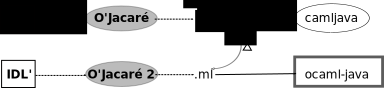
\includegraphics{schema1.pdf}

\subsection{travail effectué (en conséquence ou non)}





\end{document}
